\chapter{Theorie}
\label{cha:Theorie}
$\gamma$-Spektroskopie beschäftigt sich allgemein mit der Interaktion von $\gamma$-Quanten mit Materie. Damit solche Wechselwirkungen wissenschaftlich untersucht und erforscht werden
können ist es grundlegend notwendig zu wissen, welchen $\gamma$-Strahler in welchen Wellenlängen emmitieren, also kurzgefasst das Spektrum eines Strahlers zu kennen. Dazu wurden 
und werden Detektoren konstruiert, welche genau diese Spektren messen sollen. In diesem Versuch ist der Germanium Detektor von Interessse. Um zu verstehen, wie dieser Detektor 
ein Spektrum misst ist es notwendig die fundamentalen Licht-Materie-Wechselwirkungen zur verstehen. Dabei dominieren für $\gamma$-Quanten allerdings schon einige wenige.

\section{Licht-Materie-Wechselwirkungen}
\label{sec:WW}
Trifft ein Photon beliebiger Energie $E = \mathrm{h}\nu$ auf einen Atom können eine hand voll Effekte auftreten. Dabei existieren drei verschiedene Interaktionspartner in einem Atom. 
Das Photon kann entweder mit Elektronen, dem Kern oder dem elektrischen Feld des Atoms wechselwirken. Bei jeder Wechselwirkung (WW) können drei unterschiedliche \enquote{Endzustände}
für das Photon auftreten. Es kann annihiliert oder gestreut werden. Bei der Streuung werden zwei fälle unterschieden. Es kann elastisch oder inelastisch gestreut werden. 
In der Tabelle in Abbildung \ref{fig:WW_photon} werden (fast) alle möglichen Wechselwirkungsprozesse genannt.

\begin{figure}
    \centering
    \includegraphics[width = \textwidth]{content/pics/tabelleGamma.png}
    \caption{Darstellung der möglichen Licht-Materie-Wechselwirkungsprozesse.}
    \label{fig:WW_photon}
\end{figure}

Dabei hängt es von der Energie des einfallenden Photons und vom \enquote{Zufall} ab welcher Prozess stattfindet. Zufall meint dabei, dass das Geschehniss statistisch verteilt ist und 
lediglich eine Abschätzung/Bestimmung der Wahrscheinlichkeit Aufschluss darüber gibt wie die Häufigkeit der Prozesse verteilt ist. Ein Maß für diese Wahrscheinlichkeit ist der
Wirkunsquerschnitt (WQ) $\sigma(E)$. Im Germanium Detektor sollen $\gamma$-Quanten gemessen gemessen werden. Für diesen Spektralbereich und im Falle von Germanium, welches die Ordnungszahl
$Z = 32$ hat, ist der gesamte Extinktionskoeffizient in Abbildung \ref{fig:germanium_wq} dargestellt. 

\begin{figure}
    \centering
    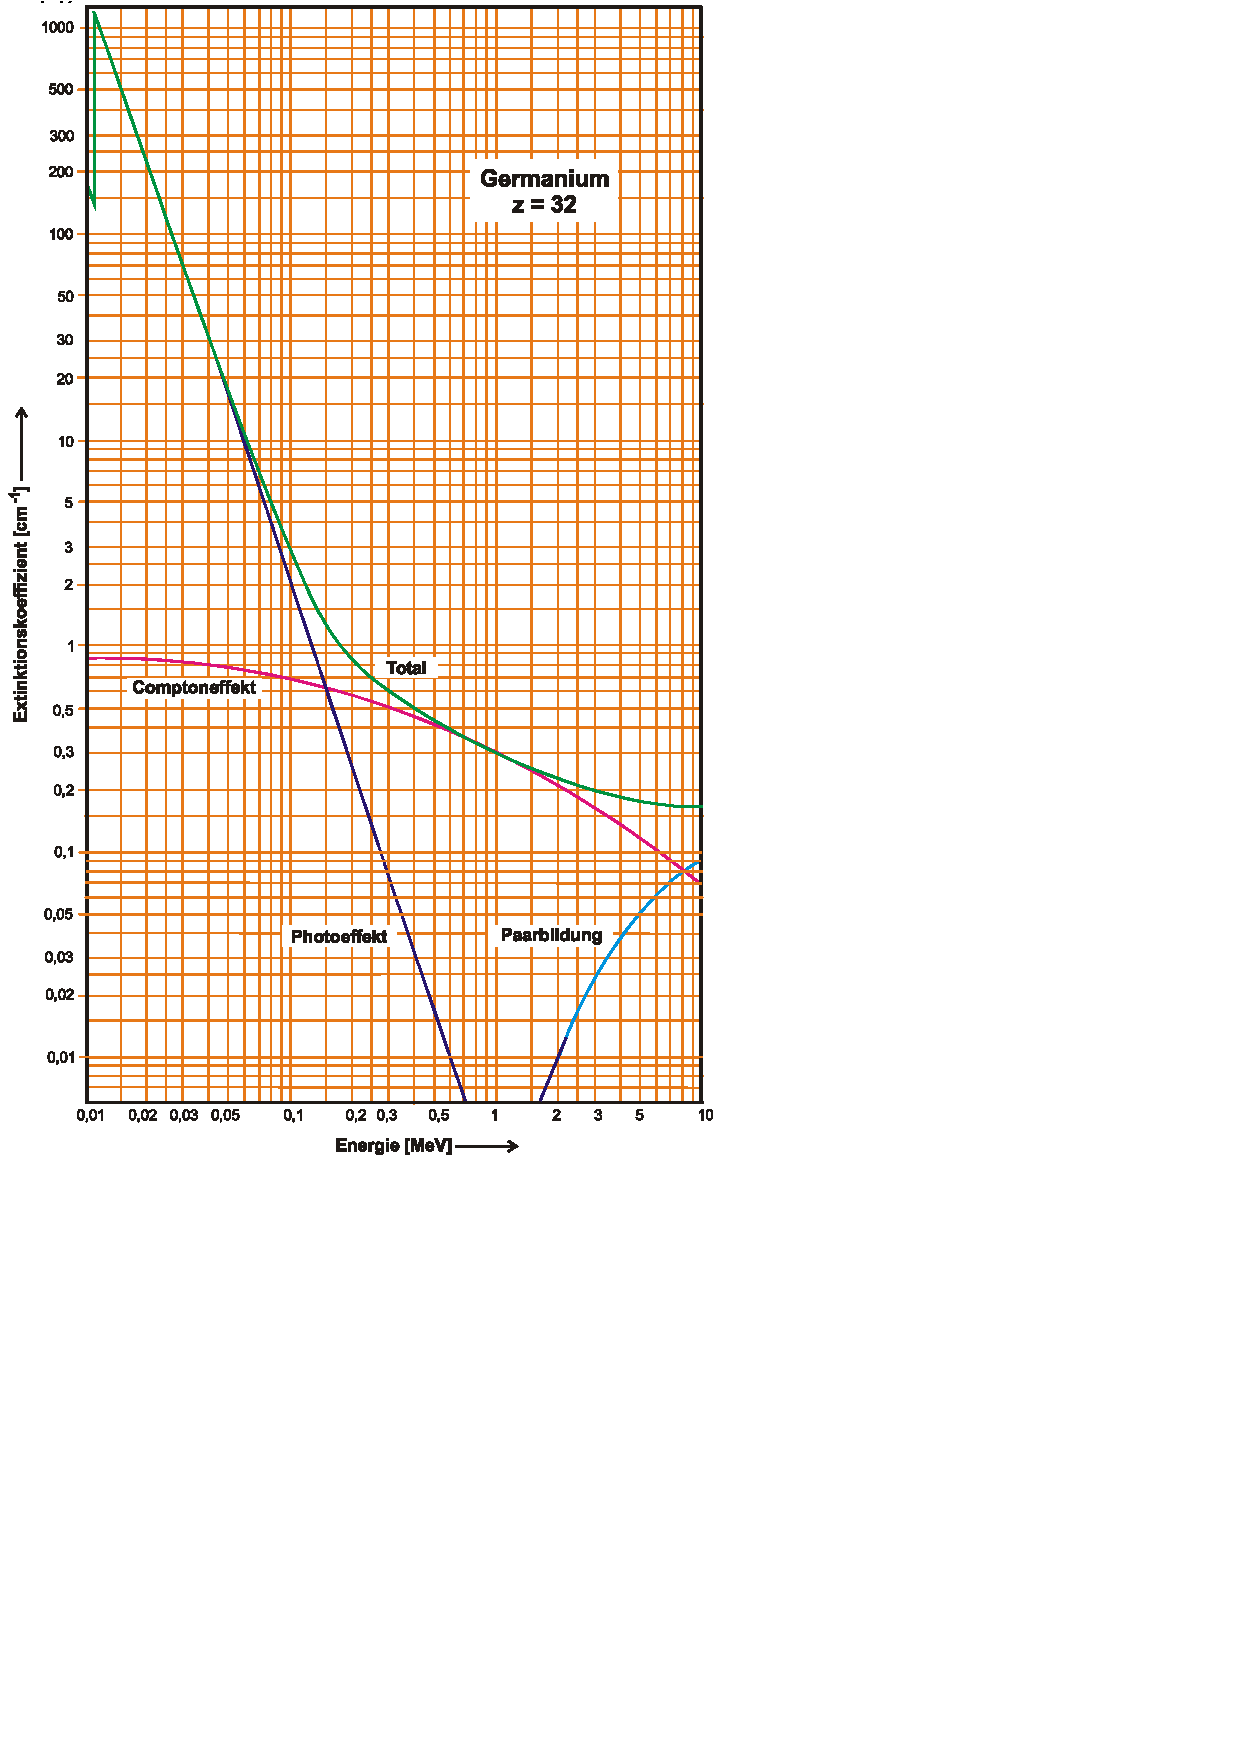
\includegraphics[height = \textheight]{content/pics/wq_germanium.pdf}
    \caption{Totaler Wirkunsquerschnitt von Germanium.}
    \label{fig:germanium_wq}
\end{figure}

Wie in Abbildung \ref{fig:germanium_wq} gezeigt, dominieren für $\gamma$-Quanten drei Effekte. Der Photoeffekt, Compton-Effekt und die Paarbildung, welche dann durch überlagerung 
den totalen WQ ergeben. Dies bedeutet, dass die anderen genannten Effekte vernachässigbar klein sind und im WQ gar nicht betrachtet werden. In diesem Versuch werden lediglich 
Strahler verwendet, welche ein Spektrum bis zu $\qty{1}{\mega\electronvolt}$ haben. Daher kann für diesen Versuch die Paarbildung ignoriert werden. Es finden also maßgeblich 
zwei Effekte statt.

\subsection{Photoeffekt}
\label{subsec:photoeffekt}
Wie Abbildung \ref{fig:WW_photon} zu entnehmen ist wird das Photon bei diesem Prozess vollständig annihiliert. Dabei transferiert es seine gesamte Energie an das Elektron.
Beim äußeren Photoeffekt interagiert das Photon mit einem Valenzelektron. Der Energieübertrag des Photons muss mindestens gleich der Bindungsenergie des Elektrons sein, sodass 
das Elektron aus der Schale herausgelößt wird. Die restliche Energiedifferenz $\Delta E = E_{\gamma} - E_{\mathrm{B}}$ erhält das Elektron als kinetische Energie. Dabei ist 
$E_{\gamma}$ die Energie des Photons und $E_{\mathrm{B}}$ die Bindungsenergie der Schale des Elektrons. Tritt nun aber der innere Photoeffekt auf, das heißt es wird nicht das 
äußere Valanzelektron, sondern ein Elektron der inneren geschlossenen Schalen ausgelöst, verbleibt ein Loch in jener Schale. Da sich das Atom in den energetisch günstigsten 
Zustand begeben wird, fällt ein äußeres Elektron in dieses Loch zurück. Dabei wird die Differenzenergie der Schalen als Photon emittiert. Dieses Photon kann natürlich auch 
wieder wechselwirken, allerdings hat es eine geringere Energie als das \enquote{erste} Photon. Nachdem durch den Photoeffekt ein Elektron ausgetreten ist und sich mit seiner
kinetischen Energie durch den Detektor bewegt, kann es weitere Elektronen durch Stöße anregen. Bei einer solchen Anregung treten die Elektronen von ihrem Valanzband in das 
Leitungsband. Durch die Wechselwirkungen wird beim Photoeffekt fast die ganze Energie im Detektor deponiert. Gerade im Germanium Detektor ist der Photoeffekt relevant, da der WQ
$\propto Z^3$ ist. Da der Photoeffekt die Qualität des Detektors stark anhebt, ist Germanium besser geeignet als Silizium, obgleich dieses günstiger wäre.

\subsection{Compton-Effekt}
\label{subsec:comptoneffekt}
Beim Compton-Effekt handelt es sich um eine inelastische Streuung an einem quasi-freien Elektron. Das Photon gibt dabei einen Teil seiner Energie an das Elektron ab und ändert 
seine Ausbreitungsrichtung. Ein einfallendes Photon der Energie $E_{\gamma}$ hat nach der Compton-Wechselwirkung die Energie 

\begin{equation}
    \label{eqn:E_compton}
    E_{\gamma}' = E_{\gamma}\frac{1}{1+\epsilon(1-\cos(\theta))}.
\end{equation}

Dabei ist $\epsilon = \sfrac{E_{\gamma}}{m_{\mathrm{e,0}}c^2}$ und $\theta$ der Streuwinkel des Photons. Die Energie des Elektrons ergibt sich aus 
\begin{equation}
    \label{eqn:E_elek_compton}
    E_\mathrm{e} = E_{\gamma} - E_{\gamma}' = E_{\gamma}\frac{\epsilon(1-\cos(\theta))}{1+\epsilon(1-\cos(\theta))}.
\end{equation}

Anhand von Gleichung \ref{eqn:E_compton} ist zu erkennen, dass der maximale Energieübertrag bei einem Streuwinkel von $\Theta = \qty{180}{\degree}$ stattfindet.
Der differentielle Wirkungsquerschnitt des Comptoneffekts ist durch 
\begin{equation}
    \label{eqn:WQ_compton}
    \frac{\mathrm{d}\sigma}{\mathrm{d}E} = \frac{3}{8}\frac{\sigma_\mathrm{Th}}{m_{\mathrm{e,0}}c^2\epsilon^2}\left(2+\left(\frac{E}{E_{\gamma} - E}\right)^2\left(\epsilon^{-2}+\frac{E_{\gamma} - E}{E}-\frac{2}{\epsilon}\left(\frac{E_{\gamma} - E}{E}\right)\right)\right).
\end{equation}

Dabei ist $\sigma_\mathrm{Th}$ der Thomson-wirkungsquerschnitt.

\section{Germanium Detektor}
\label{sec:germanium_detektor}
Der Germanium Detektor ist wie eine einfache Diode aufgebaut. 
%als nächstes hier erstmal den aufbau erklären und pdf croppen auser anleitung. dann erklären wie die dotierung geschieht. dann erklären wie der detektor miss. auf verstärker eingehen. und dann auf kenngößen und sowas